% !TEX program = xelatex
\documentclass[tikz,border=9pt]{standalone}
\usepackage[T1]{fontenc}
\usepackage{newtxtext,newtxmath}
\usepackage{tikz}
\usetikzlibrary{arrows.meta,positioning,fit,calc,backgrounds}

\hyphenpenalty=10000
\exhyphenpenalty=10000

\begin{document}
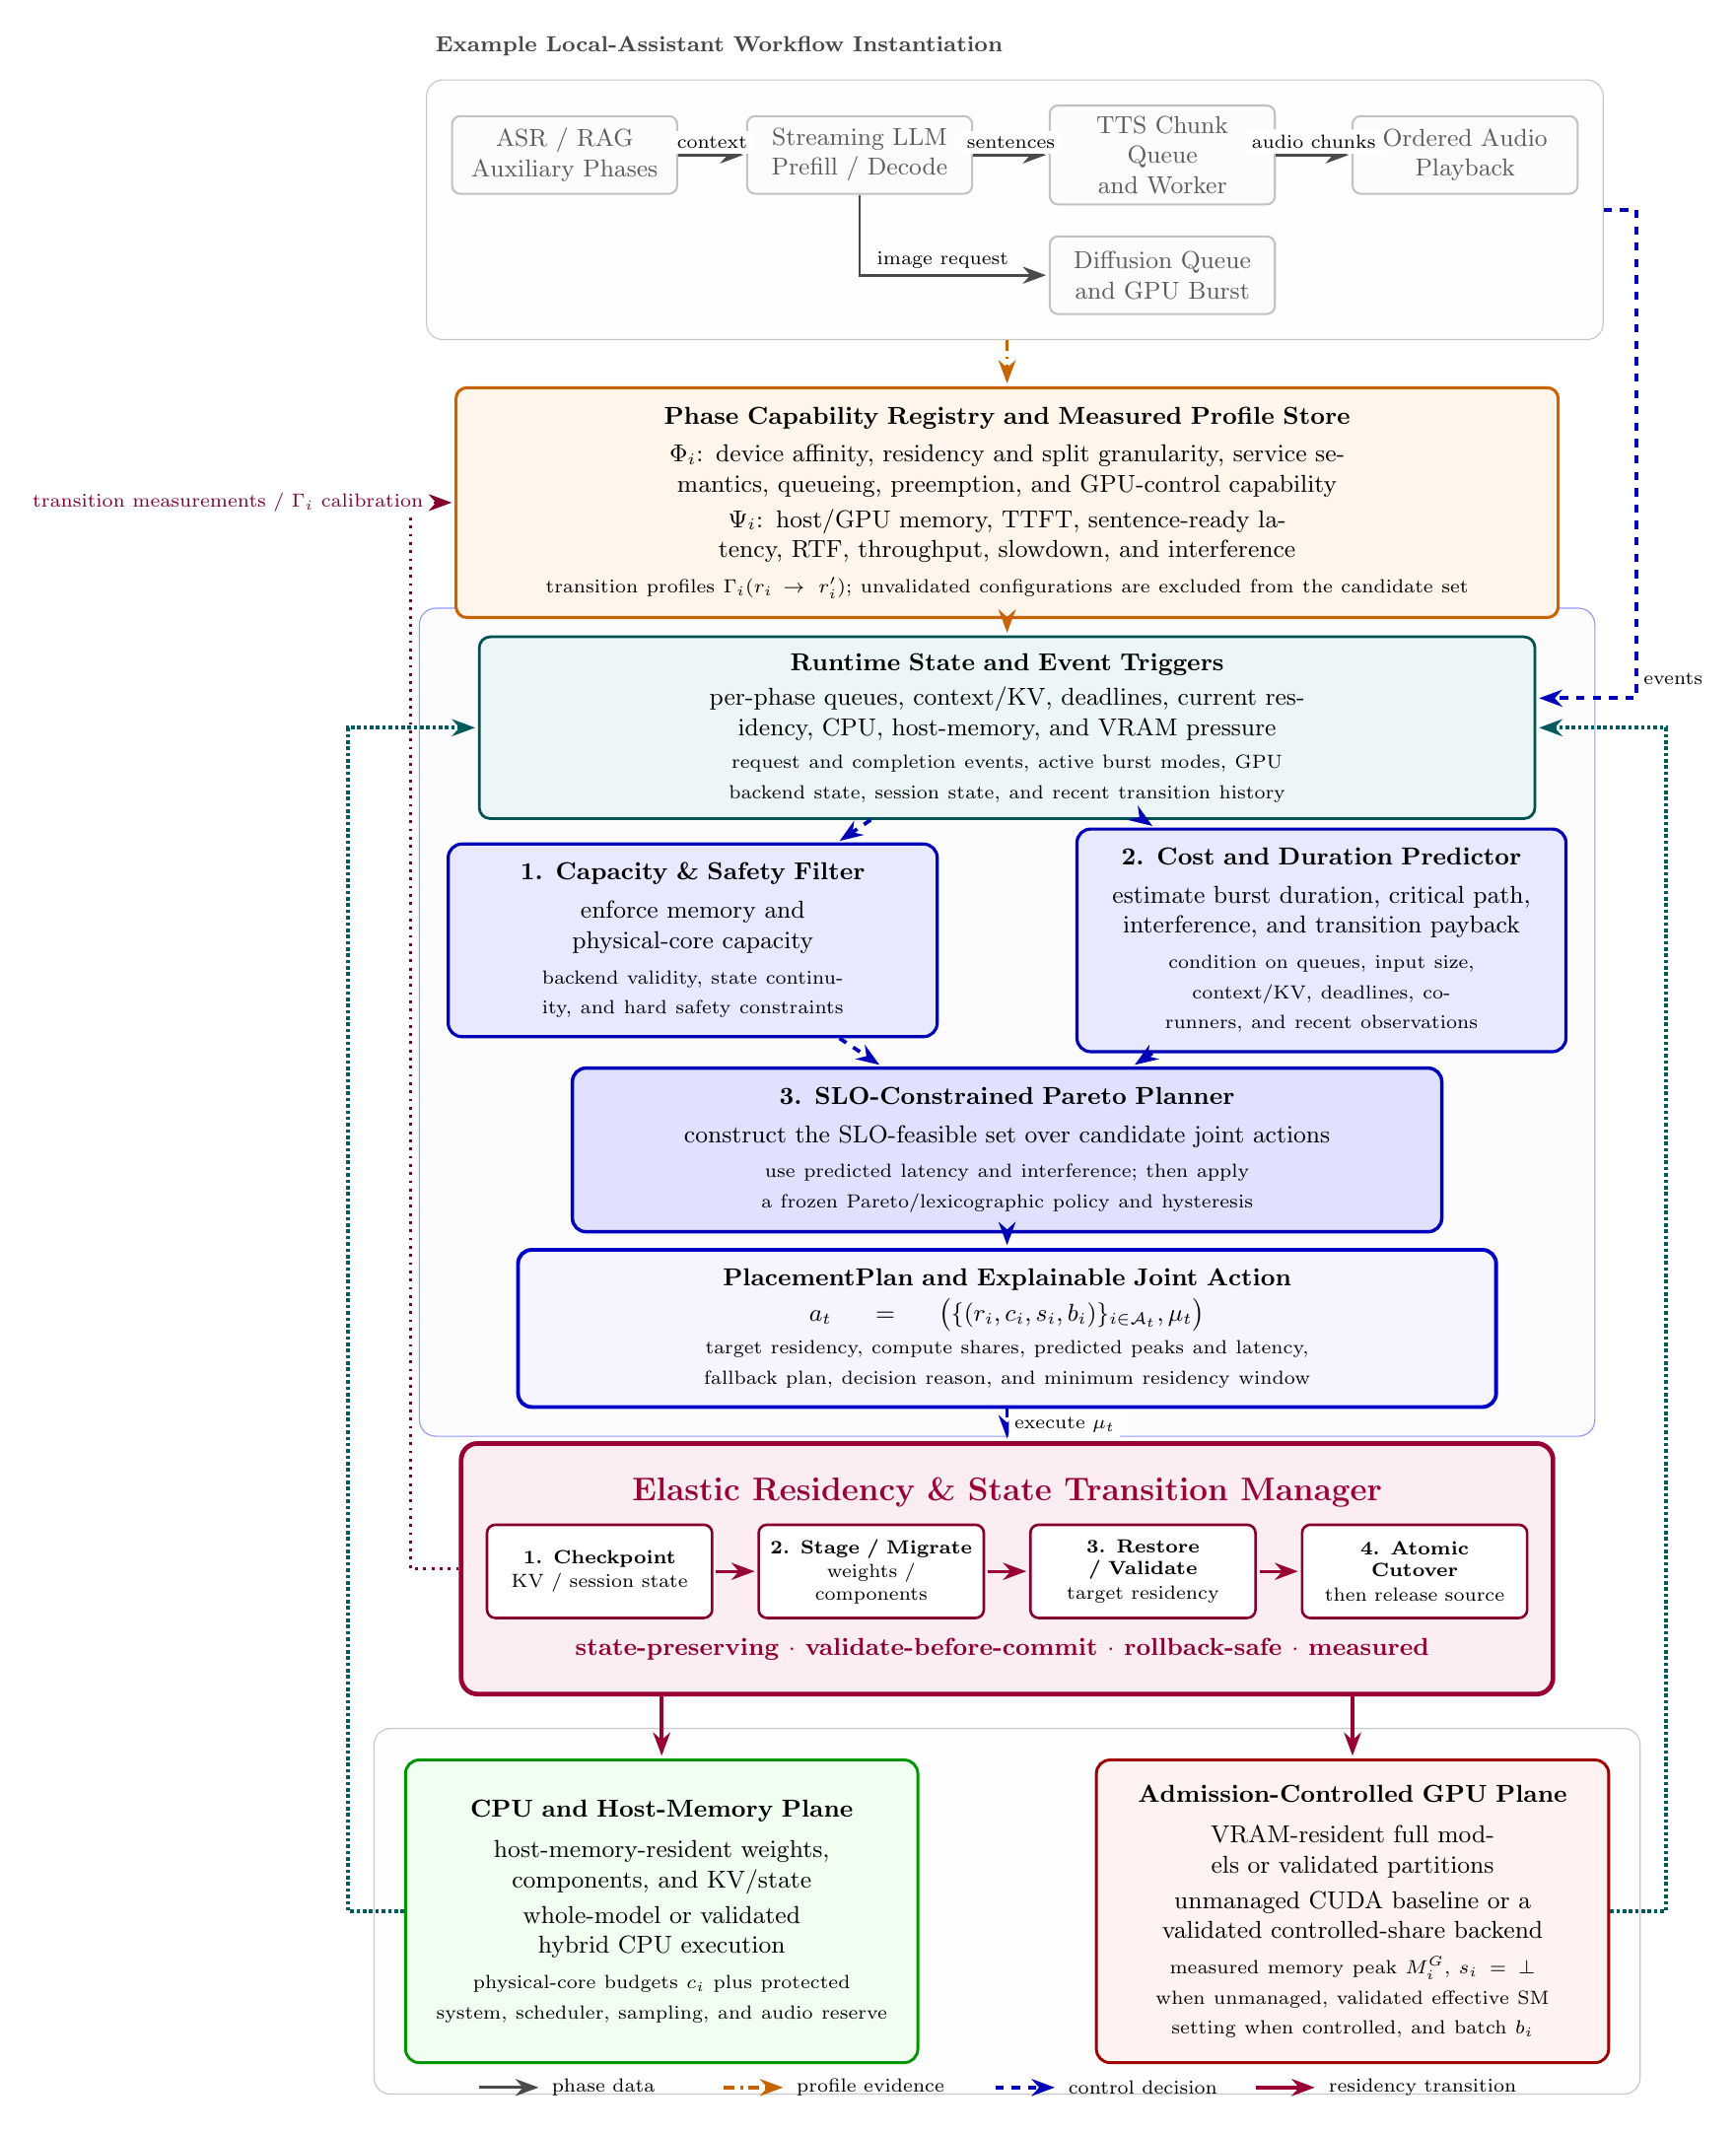
\begin{tikzpicture}[
    >={Stealth[length=3.0mm,width=2.2mm]},
    font=\small,
    phase/.style={
        draw=gray!48,
        fill=gray!2,
        text=gray!72!black,
        rounded corners=3pt,
        line width=0.75pt,
        minimum width=29mm,
        minimum height=10mm,
        text width=26mm,
        align=center,
        inner sep=4pt
    },
    knowledge/.style={
        draw=orange!78!black,
        fill=orange!8,
        rounded corners=4pt,
        line width=1.1pt,
        minimum width=142mm,
        minimum height=20mm,
        text width=135mm,
        align=center,
        inner sep=7pt
    },
    state/.style={
        draw=teal!65!black,
        fill=teal!7,
        rounded corners=4pt,
        line width=1.0pt,
        minimum width=136mm,
        minimum height=18mm,
        text width=129mm,
        align=center,
        inner sep=6pt
    },
    decision/.style={
        draw=blue!72!black,
        fill=blue!9,
        rounded corners=5pt,
        line width=1.15pt,
        minimum width=63mm,
        minimum height=24mm,
        text width=57mm,
        align=center,
        inner sep=7pt
    },
    selector/.style={
        draw=blue!72!black,
        fill=blue!12,
        rounded corners=5pt,
        line width=1.25pt,
        minimum width=112mm,
        minimum height=19mm,
        text width=105mm,
        align=center,
        inner sep=7pt
    },
    plan/.style={
        draw=blue!78!black,
        fill=blue!4,
        rounded corners=5pt,
        line width=1.4pt,
        minimum width=126mm,
        minimum height=18mm,
        text width=119mm,
        align=center,
        inner sep=7pt
    },
    managerstep/.style={
        draw=purple!70!black,
        fill=white,
        rounded corners=3pt,
        line width=0.95pt,
        minimum width=29mm,
        minimum height=12mm,
        text width=26mm,
        align=center,
        font=\scriptsize,
        inner sep=4pt
    },
    managerbox/.style={
        draw=purple!80!black,
        fill=purple!7,
        rounded corners=6pt,
        line width=1.7pt,
        inner sep=9pt
    },
    hostpool/.style={
        draw=green!58!black,
        fill=green!6,
        rounded corners=5pt,
        line width=1.05pt,
        minimum width=66mm,
        minimum height=39mm,
        text width=59mm,
        align=center,
        inner sep=8pt
    },
    gpupool/.style={
        draw=red!62!black,
        fill=red!5,
        rounded corners=5pt,
        line width=1.05pt,
        minimum width=66mm,
        minimum height=39mm,
        text width=59mm,
        align=center,
        inner sep=8pt
    },
    dataflow/.style={
        ->,
        draw=gray!58!black,
        line width=1.0pt,
        shorten >=1pt
    },
    profileflow/.style={
        ->,
        draw=orange!78!black,
        dash pattern=on 4pt off 2pt on 1pt off 2pt,
        line width=1.3pt,
        shorten >=1pt
    },
    control/.style={
        ->,
        draw=blue!72!black,
        dashed,
        line width=1.35pt,
        shorten >=1pt
    },
    feedback/.style={
        ->,
        draw=teal!72!black,
        densely dotted,
        line width=1.3pt,
        shorten >=1pt
    },
    transitionflow/.style={
        ->,
        draw=purple!80!black,
        line width=1.55pt,
        shorten >=1pt
    },
    managerflow/.style={
        ->,
        draw=purple!80!black,
        line width=1.2pt,
        shorten <=1pt,
        shorten >=1pt
    },
    profileupdate/.style={
        ->,
        draw=purple!68!black,
        dash pattern=on 1pt off 2pt,
        line width=0.95pt,
        preaction={draw=white,line width=3.0pt},
        shorten >=1pt
    },
    edgelabel/.style={
        fill=white,
        rounded corners=1pt,
        inner sep=2pt,
        align=center,
        font=\scriptsize
    }
]

% ------------------------------------------------------------------
% Example workflow instantiation
% ------------------------------------------------------------------
\node[phase] (aux) at (-5.7,13.2) {ASR / RAG\\Auxiliary Phases};
\node[phase] (llm) at (-1.9,13.2) {Streaming LLM\\Prefill / Decode};
\node[phase] (tts) at (2.0,13.2) {TTS Chunk Queue\\and Worker};
\node[phase] (playback) at (5.9,13.2) {Ordered Audio\\Playback};
\node[phase] (diffusion) at (2.0,11.65) {Diffusion Queue\\and GPU Burst};

\draw[dataflow] (aux) -- node[edgelabel,above] {context} (llm);
\draw[dataflow] (llm) -- node[edgelabel,above] {sentences} (tts);
\draw[dataflow] (tts) -- node[edgelabel,above] {audio chunks} (playback);
\draw[dataflow] (llm.south) |- node[edgelabel,pos=0.72,above]
    {image request} (diffusion.west);

\begin{pgfonlayer}{background}
    \node[
        draw=gray!45,
        fill=gray!1,
        rounded corners=6pt,
        inner sep=9pt,
        fit=(aux)(llm)(tts)(playback)(diffusion)
    ] (workflowbg) {};
\end{pgfonlayer}

\node[font=\footnotesize\bfseries,text=gray!55!black,anchor=south west]
    at ($(workflowbg.north west)+(0,0.18)$)
    {Example Local-Assistant Workflow Instantiation};

% ------------------------------------------------------------------
% Profile evidence and scheduler
% ------------------------------------------------------------------
\node[knowledge] (profiles) at (0,8.72) {
    \textbf{Phase Capability Registry and Measured Profile Store}\\[3pt]
    {\small $\Phi_i$: device affinity, residency and split granularity,
    service semantics, queueing, preemption, and GPU-control capability}\\[2pt]
    {\small $\Psi_i$: host/GPU memory, TTFT, sentence-ready latency, RTF,
    throughput, slowdown, and interference}\\[2pt]
    {\scriptsize transition profiles $\Gamma_i(r_i\!\rightarrow r_i')$;
    unvalidated configurations are excluded from the candidate set}
};

\node[state] (state) at (0,5.82) {
    \textbf{Runtime State and Event Triggers}\\[2pt]
    {\small per-phase queues, context/KV, deadlines, current residency,
    CPU, host-memory, and VRAM pressure}\\[1pt]
    {\scriptsize request and completion events, active burst modes,
    GPU backend state, session state, and recent transition history}
};

\node[decision] (capacity) at (-4.05,3.08) {
    \textbf{1. Capacity \& Safety Filter}\\[3pt]
    {\small enforce memory and physical-core capacity}\\[2pt]
    {\scriptsize backend validity, state continuity,
    and hard safety constraints}
};

\node[decision] (predictor) at (4.05,3.08) {
    \textbf{2. Cost and Duration Predictor}\\[3pt]
    {\small estimate burst duration, critical path, interference,
    and transition payback}\\[2pt]
    {\scriptsize condition on queues, input size, context/KV,
    deadlines, co-runners, and recent observations}
};

\node[selector] (selector) at (0,0.38) {
    \textbf{3. SLO-Constrained Pareto Planner}\\[3pt]
    {\small construct the SLO-feasible set over candidate joint actions}\\[2pt]
    {\scriptsize use predicted latency and interference; then apply a frozen
    Pareto/lexicographic policy and hysteresis}
};

\node[plan] (plan) at (0,-1.92) {
    \textbf{PlacementPlan and Explainable Joint Action}\\[2pt]
    {$a_t=\bigl(\{(r_i,c_i,s_i,b_i)\}_{i\in\mathcal A_t},\mu_t\bigr)$}\\[1pt]
    {\scriptsize target residency, compute shares, predicted peaks and latency,
    fallback plan, decision reason, and minimum residency window}
};

\draw[profileflow] (workflowbg.south -| profiles.north) -- (profiles.north);
\draw[control] (workflowbg.east) -- ++(0.42,0) |-
    node[edgelabel,pos=0.48,right] {events}
    ($(state.east)+(0,0.38)$);
\draw[profileflow] (profiles) -- (state);
\draw[control] (state) -- (capacity);
\draw[control] (state) -- (predictor);
\draw[control] (capacity) -- (selector);
\draw[control] (predictor) -- (selector);
\draw[control] (selector) -- (plan);

\begin{pgfonlayer}{background}
    \node[
        draw=blue!42,
        fill=blue!1,
        rounded corners=6pt,
        inner sep=10pt,
        fit=(state)(capacity)(predictor)(selector)(plan)
    ] (schedulerbg) {};
\end{pgfonlayer}

% ------------------------------------------------------------------
% Elastic residency and state-transition manager
% ------------------------------------------------------------------
\node[font=\large\bfseries,text=purple!80!black]
    (managertitle) at (0,-4.03)
    {Elastic Residency \& State Transition Manager};

\node[managerstep] (checkpoint) at (-5.25,-5.05) {
    \textbf{1. Checkpoint}\\[1pt]
    KV / session state
};
\node[managerstep] (stage) at (-1.75,-5.05) {
    \textbf{2. Stage / Migrate}\\[1pt]
    weights / components
};
\node[managerstep] (restore) at (1.75,-5.05) {
    \textbf{3. Restore / Validate}\\[1pt]
    target residency
};
\node[managerstep] (cutover) at (5.25,-5.05) {
    \textbf{4. Atomic Cutover}\\[1pt]
    then release source
};

\draw[managerflow] (checkpoint) -- (stage);
\draw[managerflow] (stage) -- (restore);
\draw[managerflow] (restore) -- (cutover);

\node[font=\small\bfseries,text=purple!75!black,align=center]
    (managerfooter) at (0,-6.05) {
    state-preserving $\cdot$ validate-before-commit $\cdot$
    rollback-safe $\cdot$ measured
};

\begin{pgfonlayer}{background}
    \node[managerbox,fit=(managertitle)(checkpoint)(stage)(restore)(cutover)(managerfooter)]
        (manager) {};
\end{pgfonlayer}

\draw[control] (plan.south) --
    node[edgelabel,right] {execute $\mu_t$} (manager.north);

\draw[profileupdate] (manager.west) -- ++(-0.62,0) |-
    node[edgelabel,pos=0.72,left,text=purple!68!black]
    {transition measurements / $\Gamma_i$ calibration} (profiles.west);

% ------------------------------------------------------------------
% Heterogeneous execution plane
% ------------------------------------------------------------------
\node[hostpool] (host) at (-4.45,-9.43) {
    \textbf{CPU and Host-Memory Plane}\\[4pt]
    {\small host-memory-resident weights, components, and KV/state}\\[2pt]
    {\small whole-model or validated hybrid CPU execution}\\[2pt]
    {\scriptsize physical-core budgets $c_i$ plus protected system,
    scheduler, sampling, and audio reserve}
};

\node[gpupool] (gpu) at (4.45,-9.43) {
    \textbf{Admission-Controlled GPU Plane}\\[4pt]
    {\small VRAM-resident full models or validated partitions}\\[2pt]
    {\small unmanaged CUDA baseline or a validated controlled-share backend}\\[2pt]
    {\scriptsize measured memory peak $M_i^G$, $s_i=\bot$ when unmanaged,
    validated effective SM setting when controlled, and batch $b_i$}
};

\draw[transitionflow] (manager.south -| host.north) -- (host.north);
\draw[transitionflow] (manager.south -| gpu.north) -- (gpu.north);

\draw[feedback] (host.west) -- ++(-0.72,0) |- (state.west);
\draw[feedback] (gpu.east) -- ++(0.72,0) |- (state.east);

\begin{pgfonlayer}{background}
    \node[
        draw=gray!45,
        fill=gray!1,
        rounded corners=6pt,
        inner sep=11pt,
        fit=(host)(gpu)
    ] (executionbg) {};
\end{pgfonlayer}

% ------------------------------------------------------------------
% Flow legend
% ------------------------------------------------------------------
\coordinate (legendbase) at (0,-11.70);
\draw[dataflow] ($(legendbase)+(-6.8,0)$) -- ++(0.8,0)
    node[right,font=\scriptsize,text=black] {phase data};
\draw[profileflow] ($(legendbase)+(-3.65,0)$) -- ++(0.8,0)
    node[right,font=\scriptsize,text=black] {profile evidence};
\draw[control] ($(legendbase)+(-0.15,0)$) -- ++(0.8,0)
    node[right,font=\scriptsize,text=black] {control decision};
\draw[transitionflow] ($(legendbase)+(3.20,0)$) -- ++(0.8,0)
    node[right,font=\scriptsize,text=black] {residency transition};

\end{tikzpicture}
\end{document}